\documentclass[class=article, crop=false]{standalone}
\usepackage[margin=1in]{geometry}
\usepackage[linesnumbered,ruled,vlined]{algorithm2e}
\usepackage{amsfonts}
\usepackage{amsmath}
\usepackage{amssymb}
\usepackage{amsthm}
\usepackage{enumitem}
\usepackage{fancyhdr}
\usepackage{hyperref}
\usepackage{minted}
\usepackage{multicol}
\usepackage{pdfpages}
\usepackage{standalone}
\usepackage[many]{tcolorbox}
\usepackage{tikz-cd}
\usepackage{transparent}
\usepackage{xcolor}
% \tcbuselibrary{minted}

\author{Nathan Solomon}

\newcommand{\fig}[1]{
    \begin{center}
        \includegraphics[width=\textwidth]{#1}
    \end{center}
}

% Math commands
\renewcommand{\d}{\mathrm{d}}
\DeclareMathOperator{\id}{id}
\DeclareMathOperator{\im}{im}
\DeclareMathOperator{\proj}{proj}
\DeclareMathOperator{\Span}{span}
\DeclareMathOperator{\Tr}{Tr}
\DeclareMathOperator{\tr}{tr}
\DeclareMathOperator{\ad}{ad}
\DeclareMathOperator{\ord}{ord}
%%%%%%%%%%%%%%% \DeclareMathOperator{\sgn}{sgn}
\DeclareMathOperator{\Aut}{Aut}
\DeclareMathOperator{\Inn}{Inn}
\DeclareMathOperator{\Out}{Out}
\DeclareMathOperator{\stab}{stab}

\newcommand{\N}{\ensuremath{\mathbb{N}}}
\newcommand{\Z}{\ensuremath{\mathbb{Z}}}
\newcommand{\Q}{\ensuremath{\mathbb{Q}}}
\newcommand{\R}{\ensuremath{\mathbb{R}}}
\newcommand{\C}{\ensuremath{\mathbb{C}}}
\renewcommand{\H}{\ensuremath{\mathbb{H}}}
\newcommand{\F}{\ensuremath{\mathbb{F}}}

\newcommand{\E}{\ensuremath{\mathbb{E}}}
\renewcommand{\P}{\ensuremath{\mathbb{P}}}

\newcommand{\es}{\ensuremath{\varnothing}}
\newcommand{\inv}{\ensuremath{^{-1}}}
\newcommand{\eps}{\ensuremath{\varepsilon}}
\newcommand{\del}{\ensuremath{\partial}}
\renewcommand{\a}{\ensuremath{\alpha}}

\newcommand{\abs}[1]{\ensuremath{\left\lvert #1 \right\rvert}}
\newcommand{\norm}[1]{\ensuremath{\left\lVert #1\right\rVert}}
\newcommand{\mean}[1]{\ensuremath{\left\langle #1 \right\rangle}}
\newcommand{\floor}[1]{\ensuremath{\left\lfloor #1 \right\rfloor}}
\newcommand{\ceil}[1]{\ensuremath{\left\lceil #1 \right\rceil}}
\newcommand{\bra}[1]{\ensuremath{\left\langle #1 \right\rvert}}
\newcommand{\ket}[1]{\ensuremath{\left\lvert #1 \right\rangle}}
\newcommand{\braket}[2]{\ensuremath{\left.\left\langle #1\right\vert #2 \right\rangle}}

\newcommand{\catname}[1]{{\normalfont\textbf{#1}}}

\newcommand{\up}{\ensuremath{\uparrow}}
\newcommand{\down}{\ensuremath{\downarrow}}

% Custom environments
\newtheorem{thm}{Theorem}[section]

\definecolor{probBackgroundColor}{RGB}{250,240,240}
\definecolor{probAccentColor}{RGB}{140,40,0}
\newenvironment{prob}{
    \stepcounter{thm}
    \begin{tcolorbox}[
        boxrule=1pt,
        sharp corners,
        colback=probBackgroundColor,
        colframe=probAccentColor,
        borderline west={4pt}{0pt}{probAccentColor},
        breakable
    ]
    \color{probAccentColor}\textbf{Problem \thethm.} \color{black}
} {
    \end{tcolorbox}
}

\definecolor{exampleBackgroundColor}{RGB}{212,232,246}
\newenvironment{example}{
    \stepcounter{thm}
    \begin{tcolorbox}[
      boxrule=1pt,
      sharp corners,
      colback=exampleBackgroundColor,
      breakable
    ]
    \textbf{Example \thethm.}
} {
    \end{tcolorbox}
}

\definecolor{propBackgroundColor}{RGB}{255,245,220}
\definecolor{propAccentColor}{RGB}{150,100,0}
\newenvironment{prop}{
    \stepcounter{thm}
    \begin{tcolorbox}[
        boxrule=1pt,
        sharp corners,
        colback=propBackgroundColor,
        colframe=propAccentColor,
        breakable
    ]
    \color{propAccentColor}\textbf{Proposition \thethm. }\color{black}
} {
    \end{tcolorbox}
}

\definecolor{thmBackgroundColor}{RGB}{235,225,245}
\definecolor{thmAccentColor}{RGB}{50,0,100}
\renewenvironment{thm}{
    \stepcounter{thm}
    \begin{tcolorbox}[
        boxrule=1pt,
        sharp corners,
        colback=thmBackgroundColor,
        colframe=thmAccentColor,
        breakable
    ]
    \color{thmAccentColor}\textbf{Theorem \thethm. }\color{black}
} {
    \end{tcolorbox}
}

\definecolor{corBackgroundColor}{RGB}{240,250,250}
\definecolor{corAccentColor}{RGB}{50,100,100}
\newenvironment{cor}{
    \stepcounter{thm}
    \begin{tcolorbox}[
        enhanced,
        boxrule=0pt,
        frame hidden,
        sharp corners,
        colback=corBackgroundColor,
        borderline west={4pt}{0pt}{corAccentColor},
        breakable
    ]
    \color{corAccentColor}\textbf{Corollary \thethm. }\color{black}
} {
    \end{tcolorbox}
}

\definecolor{lemBackgroundColor}{RGB}{255,245,235}
\definecolor{lemAccentColor}{RGB}{250,125,0}
\newenvironment{lem}{
    \stepcounter{thm}
    \begin{tcolorbox}[
        enhanced,
        boxrule=0pt,
        frame hidden,
        sharp corners,
        colback=lemBackgroundColor,
        borderline west={4pt}{0pt}{lemAccentColor},
        breakable
    ]
    \color{lemAccentColor}\textbf{Lemma \thethm. }\color{black}
} {
    \end{tcolorbox}
}

\definecolor{proofBackgroundColor}{RGB}{255,255,255}
\definecolor{proofAccentColor}{RGB}{80,80,80}
\renewenvironment{proof}{
    \begin{tcolorbox}[
        enhanced,
        boxrule=1pt,
        sharp corners,
        colback=proofBackgroundColor,
        colframe=proofAccentColor,
        borderline west={4pt}{0pt}{proofAccentColor},
        breakable
    ]
    \color{proofAccentColor}\emph{\textbf{Proof. }}\color{black}
} {
    \qed \end{tcolorbox}
}

\definecolor{noteBackgroundColor}{RGB}{240,250,240}
\definecolor{noteAccentColor}{RGB}{30,130,30}
\newenvironment{note}{
    \begin{tcolorbox}[
        enhanced,
        boxrule=0pt,
        frame hidden,
        sharp corners,
        colback=noteBackgroundColor,
        borderline west={4pt}{0pt}{noteAccentColor},
        breakable
    ]
    \color{noteAccentColor}\textbf{Note. }\color{black}
} {
    \end{tcolorbox}
}


\fancyhf{}
\lhead{Nathan Solomon}
\rhead{Page \thepage}
\pagestyle{fancy}

\begin{document}
\section{4/30/2024 lecture}
\subsection{The greenhouse effect}
Without the greenhouse effect, Earth would be too cold for life to exist. The greenhouse effect is when visible light from the sun passes through our atmosphere, is absorbed by the ground and reemitted as infrared radiation, which greenhouse gases in our atmosphere can absorb.
\par
A ``greenhouse gas" is any gas which can absorb infrared radiation. Gases with 2 different types of elements, like $CO_2$, $H_2O$, and $CH_4$ are all greenhouse gases. Generally, complicated molecules are greenhouse gases because they have low-energy rotational and vibrational modes that can interact with infrared photons. Diatomic oxygen and nitrogen are not greenhouse gases.
\par
Excess carbon dioxide in our atmosphere is a huge concern. The amount of $CO_2$ in the atmosphere correlates almost perfectly with global temperature over the past million years. Also, $CO_2$ dissolves into our oceans to form carbonic acid ($H_2CO_3$), which dissolves coral and shells of marine animals. The oceans are important for reducing carbon dioxide levels -- ocean plankton accounts for most of the photosynthesis on Earth.
\subsection{Geology}
\fig{xkcd_soil.png}
Another important thing to look for when searching for planets that can support life is plate textonics. This is a symptom of being ``geologically active", which is important for multiple reasons. First, it allows gases from the planet'c core to escape and form an atmosphere. Second, it brings new elements from the Earth's core to the surface. Most importantly, though, it means that there could be a dynamo effect taking place in the planets core, which could generate enough of a magnetic field to deflect deadly solar radiation. Deflecting the solar wind not only protects life on the surface, it also protects the atmosphere from being blown away (this is what happened to Mars).
\par
Here is a picture of the Aurora Borealis taken in just outside Davis, California during the solar storm in May 2024 (taken from r/UCDavis):

\begin{center}
    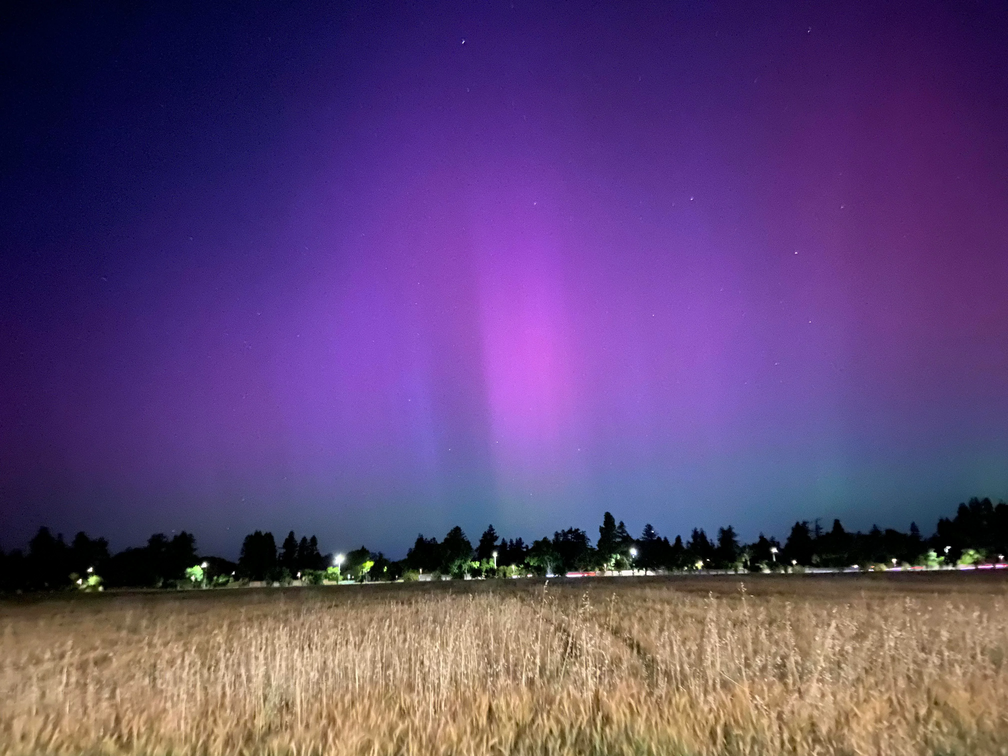
\includegraphics[width=.7\textwidth]{aurora_in_davis.png}
\end{center}
There is also a very strong dynamo effect on Jupiter, caused by fast-moving metallic hydrogen. The resulting magnetic fields are strong enough to accelerate cosmic rays, which releases radiation. Here is a picture of the magnetosphere of Jupiter (the aurora is the blue part at the top):
\fig{jupiter_aurorae.jpg}
The Earth can be split up into layers. The lithosphere includes the continental crust, the oceanic crust, and the uppermost part of the mantle. Under the crust is the mantle, which is made of minerals containing silicon and oxygen. Convection in the mantle causes plate tectonics. The heaviest elements, like nickel and iron, sink down to the core. Radioactive atoms inside the Earth add heat to the mantle. Also, planetary differentiation (the process in which heavier atoms sink to the core) adds heat, because viscous friction converts their gravitational potential energy into kinetic energy.
\par
For a sphere, the surface area divided by the volume is $3/r$, where $r$ is the radius. Therefore, smaller planets cool off faster. This is why Mercury and Mars are not geologically active, but Venus and Earth are.
\par
The carbon dioxide cycle begins with (1) atmospheric $CO_2$ dissolving into rainwater, then (2) eroding minerals and flowing into the ocean with those minerals. Then, (3) the carbon dioxide combines with those minerals to make rocks on the ocean floor, and (4) subduction carries the carbonate rocks into the mantle. Those rocks then melt and the carbon dioxide is (5) released into the atmosphere via volcanoes.
\par
The Earth has a ``natural thermostat": higher temperatures cause more precipitation, which removes carbon dioxide from the atmosphere, lowering the temperature. The opposite process also works. Since this keeps the Earth's temperature so stable, we don't know what caused the ice ages, but we think it may have been variations in our axial tilt.
\subsection{Meteoroids}
The dinosaurs were wiped out 65 million years ago by the K-T extinction, which was triggered by an asteroid collision. Scientists have found a thin 65 million year old layer of iridium all over the planet. This is because iridium is common in meteorites but extremely rare on Earth. The particular asteroid that cause the K-T extinction was about 10 km in diameter, hit hear the Yucatán peninsula, and released enough debris to block a decent amount of sunlight. That lack of sunlight made the world temporarily extra cold, which is why so many species went extinct. Nuclear war could do the same thing by releasing a ton of dust into the atmosphere. This is what we call a ``nuclear winter".
\par
In 2013, in asteroid detonated in the sky above Chelyabinsk, Russia, releasing as much energy as 500 kilotons of TNT (The Little Boy in Hiroshima and the Fat Man in Nagasaki were 15 and 21 kilotons, respectively). The shock wave injured 1400 people and damaged 7200 buildings.
\par
The frequency of meteors is roughly inversely proportional to the size of the meteor -- this is sort of like saying meteors follow Zipf's law. Thankfully, massive meteor impacts are extremely rare. Also, thanks to people like Ned Wright at UCLA, we may have the technology now to deflect some meteors.
\par
Some scientists fear that if multiple supervolcanos on Earth go off at the same time, it could release enough greenhouse gases to set off a runaway greenhouse effect, turning us into a planet like Venus.
\par
We may be in 6th mass extinction right now due to human activity.

\subsection{Early life on Earth}
For life to exist on a planet, the planet must have nutrients, usable energy (probably in the form of sunlight or chemical potential), and liquid water. Liquid water is very hard to find.
\par
Microbial life on Earth began around 500 million years after the Earth formed, and it took another 3.5 billion years to form interesting multicellular organisms. Oxygen began to appear 2.3-2.4 billion years ago, and 500 million years ago, there was enough oxygen for animals to breathe. This set off the Cambrian explosion, when animals became much more diverse, and then plants, fungi, and animals appeared on land. Mammals and dinosaurs appeared about 200 million years ago, and hominids appeared about 1 million years ago.
\par
All of the 5 known mass extinctions occured after the Cambrian explosion (within the last 10\% of the Earth's history).

\end{document}
